\chapter{Concrete syntax}
\label{concretechapter}

\section{Introduction}

Although an abstract syntax describes the underlying vocabulary and grammar of a language, it does not define how the abstract syntax is presented to the end user, that detail is described by a concrete syntax which can either be in diagrammatic or textual form.  Many contemporary modelling languages use diagrammatic concrete syntax such as state machines and class diagrams, but diagrammatic syntaxes are often limited by the real estate of the user's display and some languages such as OCL have only a textual syntax.

Dealing with concrete syntax is a two stage process.  The first stage involves interpreting the syntax and ensuring that it is valid.  In the second stage, the concrete syntax is used to build the abstract syntax.  These stages are equally applicable to both text and diagrams although there is an important difference in the way the concrete syntaxes are constructed by the end user. Diagrams are commonly constructed interactively and therefore incrementally, consequently the syntax must be interpreted in parallel to the user's interaction.  On the other hand, textual syntax is usually interpreted in batch, the user constructs the complete model using the syntax and only then is it passed to the interpreter.  This style of processing syntax is comparable to programming language compilers and interpreters.

The first part of this chapter describes the XBNF textual parser component of XMF and demonstrates how it can be used to realise the interpreting of text based concrete syntax and the construction of the abstract syntax.  The second part of the chapter discusses how diagrammatic syntax is defined and how it is linked and synchronised with abstract syntax using XSync.

\section{Textual Syntax}

In this section we describe the parsing of text using XBNF.  The XBNF language is based on EBNF which is a popular approach to describing the grammars of languages, because of this the grammars of most textual languages are easily available (Ada, Java, SQL, for example).  Once a grammar for a language has been defined, the next step is to define how abstract syntax is constructed (or synthesised) as a result of the parsing input using the grammar.  Although the approach described in this section is oriented towards producing the type of abstract syntax structures described in chapter \ref{abschapter}, the mechanisms used are generic one and can be generally applied to a wide range of text parsing problems.

\subsection{Parsing text using EBNF}

The interpretation of textual syntax involves defining the rules by which streams of ASCII characters are deemed to be valid concrete syntax.  These rules are commonly referred to as the grammar rules of a language.  A grammar consists of a collection of clauses of the form:

\begin{verbatim}
NAME ::= RULE
\end{verbatim}

\noindent where a RULE defines how to recognise a sequence of input characters.  An example of a rule is the following:

\begin{verbatim}
Calculator ::= Mult '='
\end{verbatim}

\noindent which defines that to satisfy the rule Calculator the input characters must first satisfy Mult, which is a non-terminal because it refers to another rule, followed by a terminal \emph{'='}.  A terminal is understood to be a sequence of characters in quotes.  A Mult is a multiplicative expression possibly involving the multiplicity (*) and division (/) operators, the grammar for Mult is defined as:

\begin{verbatim}
Mult ::= Add ('*' Mult | '/' Mult)
\end{verbatim}

The rule for Mult shows a number of typical grammar features.  A Mult is successfully recognised when an Add is recognised followed by an optional \emph{'*'} or \emph{'/'} operator.  The choice is described by separating the two or more options (terminals or non-terminals) using the vertical bar.  Consequently this rule defines three possibilities:

\begin{itemize}

\item The input stream satisfies Add followed by a '*' followed by Mult.
\item The input stream satisfies Add followed by a '/' followed by Mult.
\item The input stream satisfies Add.

\end{itemize}

The grammar for Add is the same as Mult except Add recognises addition expressions:

\begin{verbatim}
Add ::=  Number ('+' Add | '-' Add)
\end{verbatim}

\subsection{Parsing text using XBNF}

XBNF augments EBNF with details concerned with managing multiple grammars.  Firstly it is necessary to put grammars somewhere so that they can be used when required, secondly it is necessary to be able to specify given an ASCII stream which grammar should be used to understand the stream.  In order to illustrate XBNF we will define the grammar for a state machine.  The following is an example of a state machine's textual concrete syntax:

\begin{lstlisting}
@StateMachine(Off)
  @State Off
  end

  @State On
  end

  @Transition(On,Off)
  end

  @Transition(Off,On)
  end
end
\end{lstlisting}\noindent As in this example, all textual syntax dealt with by XMF is littered with @ symbols.  These symbols are
special because the word immediately after the symbol indicates where the top level grammar rules can be found which validate the syntax immediately after the declaration.  In the above example, this specifies that the syntax \emph{(Off)} should be understood in the context of the grammar defined in class \emph{StateMachine}, that \emph{Off} and \emph{On} should be understood in terms of the grammar defined in the class \emph{State} and that \emph{(On,Off)} and \emph{(Off,On)} should be interpreted in the context of the grammar defined in the class \emph{Transition}.  The three classes to interpret this collective syntax is defined below\footnote{Note that \emph{Name} is a built in rule which matches any combination of alphanumeric characters}:

\begin{lstlisting}
@Class StateMachine
  @Grammar
    StateMachine ::= '(' startName = Name ')' elements = Exp*
  end
end

@Class State
  @Grammar
    State ::= name = Name
  end
end

@Class Transition
  @Grammar
    Transition ::= '(' sourceName = Name ',' targetName = Name ')'
  end
end
\end{lstlisting}\noindent The grammar rules are embedded in the body of the \emph{@Grammar}.  These say that the textual syntax for a
\emph{StateMachine} consists of a \emph{Name} (the name of the starting state) followed by zero or more \emph{Exp} referring to the whichever grammar rules parses the body of the \emph{StateMachine} (which is likely to be \emph{State} or \emph{Transition}).  A \emph{State} consists only of a \emph{Name} (its name).  A \emph{Transition} consists of two names parsing the source and target state of the transition.

The @ grammar reference symbol as a means of referring to different grammars offers massive flexibility since language grammars can be mixed.  It is possible to use the state machine language in the context of regular XOCL expressions for example (since XOCL and all XMF languages are defined using precisely the method outlined in this book).  Sometimes however the @ symbol can be inconvenient when an existing language must be parsed since the text of that language must be augmented with the @ grammar reference symbol in order to parse it using XBNF.  In this case it is possible to collectively define the grammar rules such that only a single top-level @ is required.  For instance, consider the case of the following state machine grammar definition:

\begin{lstlisting}
@Class StateMachine
  @Grammar
    StateMachine ::= '(' startName = Name ')' elements = (State | Transition)*.

    State ::= name = Name.

    Transition ::= '(' sourceName = Name ',' targetName = Name ')'.
  end
end
\end{lstlisting}\noindent This grammar will support the parsing of the following syntax which has a single @ denoting the single required rule:

\begin{lstlisting}
@StateMachine(Off)
  State Off
  end

  State On
  end

  Transition(On,Off)
  end

  Transition(Off,On)
  end
end
\end{lstlisting}\subsection{Building Abstract Syntax}

Having established whether a given textual syntax is valid, the next step is to model the construction of the abstract syntax.  The steps taken by XBNF are illustrated in figure \ref{process}.  As can be seen from this, XBNF produces XMF abstract syntax as a result of the parse and evaluates this to produce an abstract syntax model.  At first glance this may seem confusing since there are two different types of abstract syntax and an evaluation step from one to the other.  The need for this is based on the generality of the XBNF mechanisms, XBNF can be used in the context of a more conventional interpreter where textual input such as 5 + 5 evaluates to the result 10.  The grammar produces the abstract syntax of 5 + 5 and the evaluator evaluates this abstract syntax to produce the value 10.  In the definition of a model based language however, the value required from the evaluator is the model based abstract syntax of the type defined in chapter \ref{abschapter}.  In which case the grammar rules must produce XMF abstract syntax that evaluates to the value of model based abstract syntax.  To avoid confusion, for the remainder of this chapter XMF abstract syntax will be refereed to as \emph{abstract syntax} and abstract syntax model will be refereed to as \emph{abstract syntax value}.

 \begin{figure}[htb]
\begin{center}
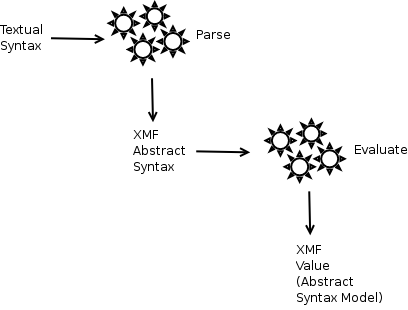
\includegraphics[width=12cm]{ConcreteSyntax/figures/process.png}
\caption{The process of translating textual syntax to model-based abstract syntax}
\label{process}
\end{center}
\end{figure}

Raw abstract syntax can be defined as a result of grammar rules however defining this can be verbose and time consuming, an alternative is to use a powerful XMF tool which eases the process of this definition.  This tool is designed around the observation that it is often the case that the required abstract syntax can be expressed in terms of an existing XMF based concrete syntax.  For example the state machine abstract syntax value described in chapter \ref{abschapter} is expressed in terms of the syntax for classes and operations.  The tool, called quasi-quoting, allows the description of new concrete syntax in terms of old concrete syntax, because most languages tend to be built from existing languages (and rarely from scratch) we deal with this method in detail in the next sections.

\subsubsection{Quasi-quoting}

Rather then describing the abstract syntax that gives rise to the abstract syntax value, quasi-quotes enables the user to instead say "give me the abstract abstract syntax that you get if you parsed this existing concrete syntax".  Quasi-quotes can be used to find the abstract syntax of any concrete textual syntax by enclosing the textual syntax as exemplified in the following way:

\begin{lstlisting}
[| ... |]
\end{lstlisting}\noindent For example, the following quasi-quotes will return the
abstract syntax for \emph{StateMachine}:

\begin{lstlisting}
[| StateMachine() |]
\end{lstlisting}Often the abstract syntax returned by quasi-quotes is not the required abstract syntax, instead it is desirable to be able to \emph{drop} values into this which have been parsed and stored by the grammar rules.  Syntactically a drop is enclosed by \emph{$<$} and \emph{$>$}.  For example, the grammar for \emph{StateMachine} parses the starting state \emph{startName} which, when evaluated to produce the abstract syntax, should be passed to the constructor of \emph{StateMachine}.  This is done in the following way (ignoring \emph{elements} for the time being):

\begin{lstlisting}
context StateMachine

@Grammar
  StateMachine ::= '(' startName = Name ')' elements = Exp {
    [| StateMachine(<startName>) end |]
  }.
end
\end{lstlisting}The same approach can be used to construct the abstract syntax for a state:

%\begin{lstlisting}
%context State
%
%@Grammar
%  State ::= name = Name action = Exp* {
%    [| State(<name>,@Operation() <action> end) end |]
%  }.
%end
%\end{lstlisting}
\begin{lstlisting}
context State

@Grammar
  State ::= name = Name {
    [| State(<name>) end |]
  }.
end
\end{lstlisting}\noindent Here the abstract syntax has the \emph{name} dropped into the quasi-quotes, and the body of an operation.  When this is evaluated to produce the abstract syntax value, these will be passed as parameters to the constructor of \emph{State}.  \emph{Transition} and \emph{StateMachine} can be defined in a similar way:

\begin{lstlisting}
context Transition

@Grammar
  Transition ::= '(' sourceName = Name ',' targetName = Name ')' {
    [| Transition(<sourceName>,<targetName>) |]
  }.
end

context StateMachine

@Grammar
  StateMachine ::= '(' startName = Name ')' elements = Exp* {
    [| StateMachine(<startName>,<elements>) |]
  }.
end
\end{lstlisting}% (To be continued with transition and returning to StateMachine to show how states and transitions are added)

\subsubsection{Sugar}

One of the side effects of using the quasi-quoting mechanism, as illustrated in the previous section, or creating abstract syntax directly, is that the original concrete syntax is lost since the translation does not record details of the original concrete syntax.   Often it is desirable to be able to make the transition back from the abstract syntax to the concrete syntax, a good example of where this is useful is during the process of debugging a model.  In order to support this XMF provides a further tool called \emph{Sugar}\footnote{The process of \emph{Sugaring} and \emph{Desugaring} (often used in programming language theory) is used to describe the process of translating to and from new syntax using existing syntax.  It captures the idea that the new syntax is not adding any fundamentally new semantics to the language, merely making existing syntax more palatable (or sweeter!) to the end user of the syntax.}.  Instead of the grammar rules constructing the abstract syntax directly, they instantiate classes of type \emph{Sugar} which then create the abstract syntax and provide methods for doing other things such as translating the consequent abstract syntax back to the concrete syntax.

An example of \emph{Sugar} class is illustrated below:

\begin{lstlisting}
@Class StateSugar extends Sugar
  @Attribute name : String end

  @Constructor(name) end

  @Operation desugar()
    [| State(<name>) |]
  end

  @Operation pprint(out,indent)
    format(out,"@State ~S",Seq{name})
  end
end
\end{lstlisting}Any class extending \emph{Sugar} must override the abstract operation \emph{desugar()} which should return the required abstract syntax.  The additional (and optional) method \emph{pprint} is used to \emph{pretty print} the original concrete syntax from the abstract syntax.  This method takes an output stream (to print the text to) and an indent variable which denotes the current indentation of the textual syntax.  In the above example, the text \emph{@State} and the state name is sent to the output stream.

The grammar rule constructs \emph{Sugar} classes as appropriate:


\begin{lstlisting}
context State
  @Grammar
    State ::= name = Name action = Exp* {
      StateSugar(name,action)
    }.
  end
\end{lstlisting}
\section{Diagrammatic Syntax}

As indicated in the introduction to this chapter, the major difference between diagrammatic syntax and textual syntax is that diagrammatic syntax is interpreted incrementally whereas textual syntax is interpreted in batch.  This presents a different set of challenges for diagrammatic syntax to that of its textual counterpart, the incremental nature of its construction must be taken into account when devising an architecture in order to support it.  A further challenge for diagrammatic languages is being able to specify the valid concrete syntax of the diagram in a
textual language such as XMF.  As we have discussed in the previous section, this is well understood for textual syntax using notations such as EBNF, but for diagrams it is less clear how the equivalent can be achieved.  In the following sections we discuss the XMF approach to doing this.

\subsection{Parsing Diagrams}

In order to describe how to interpret a diagram, we must first define what it means to be a diagram at some (useful) level of abstraction.  This is achieved by forming a model of diagrams in XMF as illustrated in figure \ref{modelOfDiagrams}, this model shares many parallels with OMG's diagram interchange model \cite{}. A key characteristics which it shares with the diagram interchange model is that its generality enables it to capture the concrete syntax concepts, and the relationship between these, for a broad spectrum of diagram types ranging from  sequence diagrams to state machines to class diagrams.

Clearly the model shown in figure \ref{modelOfDiagrams} does abstract from details that may be important such as their rendering and the paradigm of interaction that gives rise to their state being changed.  This detail is outside the scope of the model, but is an important component of realising this approach in the context of a real tooling environment.  One approach to dealing with this detail is to interface to some external tool that understands how
to render the concepts and respond to user interaction.  Since this is an implementation detail we do not dwell on it here, instead we make the assumption that the instantiating of concepts in figure \ref{modelOfDiagrams} results in the concrete display of the denoted element.  Moreover we assume that interaction with the concrete display, moving a node for example, results in the state of its model-based counterpart being updated.  A suitable implementation of this scenario can be black boxed such that new diagram types are constructed only as a result of dealing with the model.

\begin{figure}[h]
\begin{center}
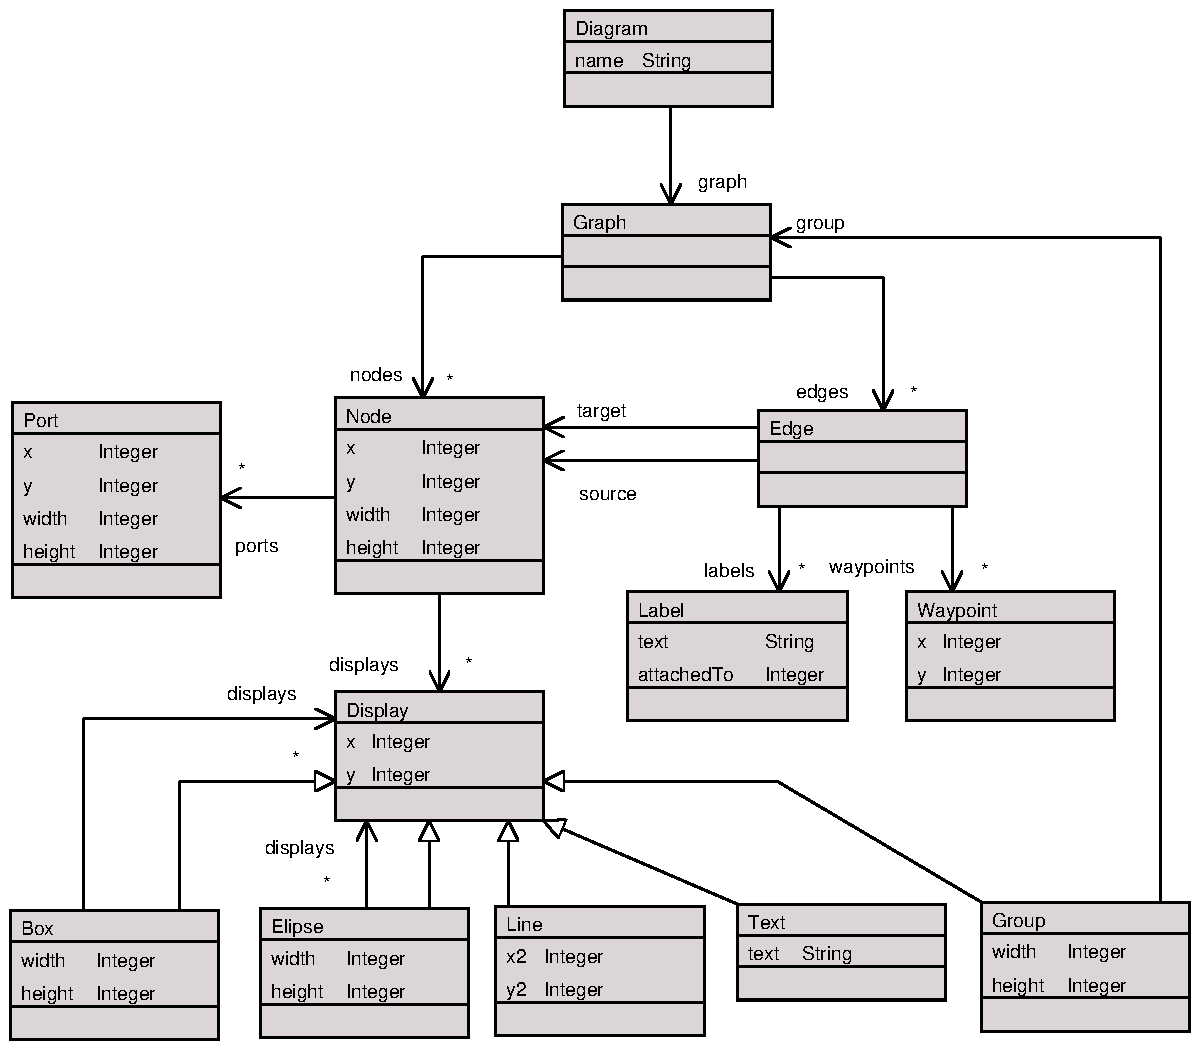
\includegraphics[width=15cm]{ConcreteSyntax/figures/diagramModel.pdf}
\caption{A model of diagrams}
\label{modelOfDiagrams}
\end{center}
\end{figure}

Specific diagramming types are described by specialising the model of diagrams, this is shown in figure \ref{stateMachineDiagram} for state machines.  In this a \emph{StateDiagram} is a type of \emph{Diagram}, the \emph{Graph} of a \emph{StateMachine} is constrained to contain \emph{TransitionEdge}s and \emph{StateNode}s
(which are specialised \emph{Edge}s and \emph{Node}s respectively). A \emph{TransitionEdge} is constrained to be the \emph{source} and \emph{target} of \emph{StateNode}s, and a \emph{StateNode} is displayed using an \emph{Elipse}.

\begin{figure}[h]
\begin{center}
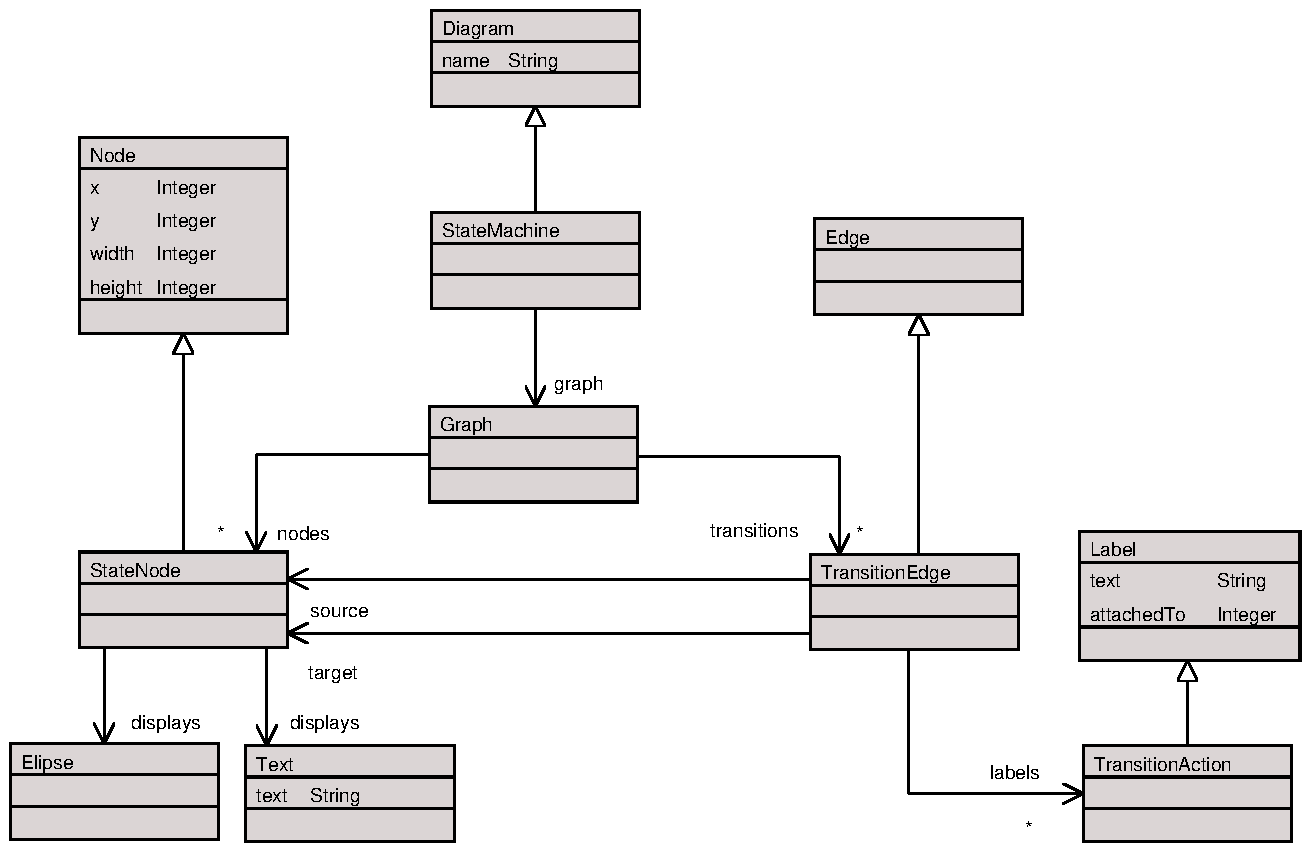
\includegraphics[width=16cm]{ConcreteSyntax/figures/stateMachineSyntax.pdf}
\caption{Specialising the model of diagrams for state machines}
\label{stateMachineDiagram}
\end{center}
\end{figure}

%\FloatBarrier

\subsection{Building Abstract Syntax}

As the user interactively constructs instances of the model of diagrams the abstract syntax should be concurrently constructed as appropriate.  One approach to achieving this is to embed operations in the concrete syntax which generate abstract syntax on the fly.  Although this approach would work well in practice, a deficiency is that it couples the abstract syntax to the concrete syntax.  In practice it may be desirable to have a single diagram
type generating different abstract syntaxes under different circumstances.  A much more flexible approach is to form a mapping between the concrete syntax and abstract syntax which neither side know about.  This scenario is illustrated in figure
\ref{uniDirMapping}.

\begin{figure}[htb]
\begin{center}
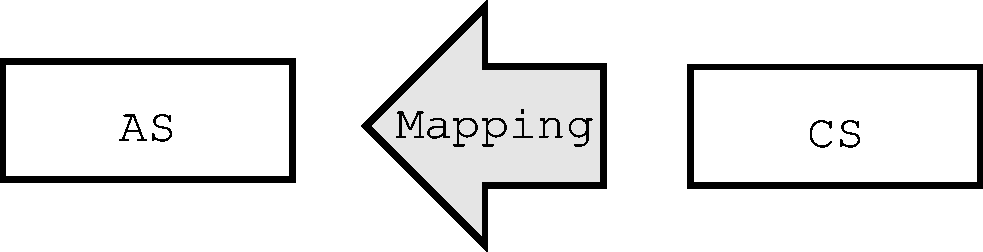
\includegraphics[width=10cm]{ConcreteSyntax/figures/uniDirMapping.pdf}
\caption{Mapping between diagram syntax and abstract syntax}
\label{uniDirMapping}
\end{center}
\end{figure}

In this the mapping listens to changes in the concrete syntax for changes that impact the abstract syntax and updates the abstract syntax appropriately.  Given a \emph{StateDiagram} and an
\emph{StateMachine}:


\begin{lstlisting}
@Class StateDiagram extends Diagram
  ...
end

@Class StateMachine

  @Attribute startName : String end
  @Attribute states : Set(State) end
  @Attribute transitions : Set(Transition) end

  ...
end
\end{lstlisting}\noindent A mapping is defined:

\begin{lstlisting}
@Class StateMachineXStateDiagram

  @Attribute statemachine      : StateMachine end
  @Attribute diagram           : StateDiagram end
  @Attribute stateMaps         : Set(StateXNode) end
  @Attribute transitionMaps    : Set(TransitionXTransitionEdge) end
  ...
\end{lstlisting}
\noindent The mapping knows about the top level constructs of the statemachine's concrete and abstract syntax.  When the mapping is constructed, a listener (or daemon) is placed on the \emph{diagram}'s graph, such that when a state added or removed, a method is invoked adding or removing a \emph{State} from the abstract syntax \emph{statemachine}:


\begin{lstlisting}
  @Constructor(statemachine,diagram)
    self.addDaemons()
  end

  @Operation checkDiagramDaemons()
    if not diagram.hasDaemonNamed("stateAdded") then
      @SlotValueChanged + stateAdded(
        diagram.graph,"nodes",newStateNode)
          self.stateNodeAdded(newStateNode)
      end
    end;
    if not diagram.hasDaemonNamed("stateRemoved") then
      @SlotValueChanged - stateRemoved(
        diagram.graph,"nodes",removedStateNode)
          self.stateNodeAdded(removedStateNode)
      end
    end
  end
\end{lstlisting}
\noindent Listeners to detect the addition and removal of transitions are implemented in a similar way.  The methods for adding and removing the \emph{State} from the \emph{statemachine} are specified as follows:

% NEED TO FIGURE OUT WHAT TO DO WITH ACTIONS


\begin{lstlisting}
  @Operation stateNodeAdded(newStateNode)
    if not stateMaps->exists(map | map.stateNode = newStateNode)
    then
      let name = self.newStateName() then
        state = State(name)
        in newStateNode.setName(name);
          self.add(StateXNode(state,newStateNode,self));
          statemachine.add(state)
      end
    end
  end

  @Operation classRemoved(class)
    @Find(map,classMaps)
      when map.class = class
      do self.remove(map);
        map.node.delete()
    end
  end
end
\end{lstlisting}
\FloatBarrier

The style of mapping concrete syntax to abstract syntax can be nested  within containership relationships such that a new mapping is generated from a listener, which in turn listens to the newly mapped elements and generates new mappings as concrete syntax elements are created ... This gives rise to the hierarchy exemplified in figure \ref{hierarchy} where only the top level mapping between concrete syntax element \emph{A} and abstract syntax element \emph{A'} is generated statically (i.e. not via listeners).

\begin{figure}[htb]
\begin{center}
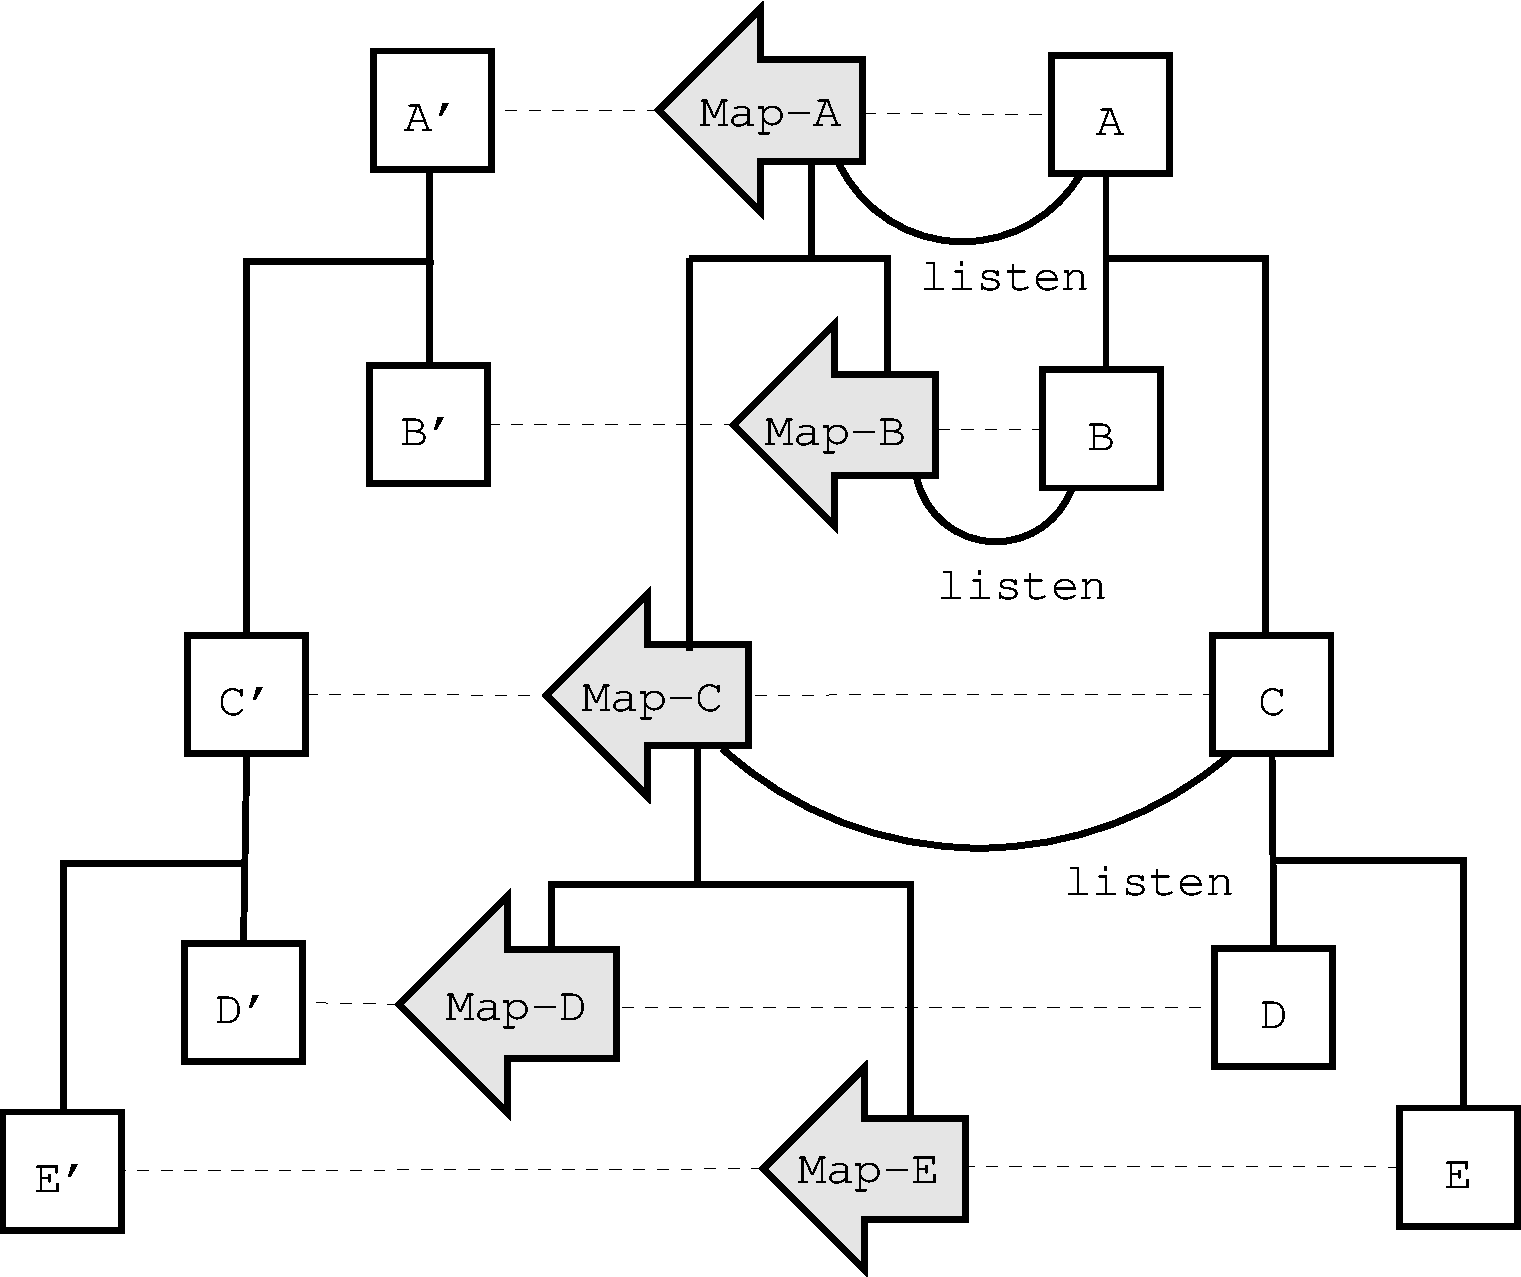
\includegraphics[width=14cm]{ConcreteSyntax/figures/containership.pdf}
\caption{An example of how listeners can generate mappings which can themselves listen and generate mappings}
\label{hierarchy}
\end{center}
\end{figure}

\subsection{Building Diagrams from Abstract Syntax}

The approach to mapping concrete syntax to abstract syntax described in the  previous section can equally be applied to the inverse mapping of abstract syntax to concrete syntax, potentially this can be done simultaneously so that changes to either side of the mapping result in an update to the other.  Such bi-directional mappings are particularly desirable in a scenario where an abstract syntax is the source of multiple concrete syntaxes (which are effectively views on the abstract syntax) a change to one concrete syntax will propagate the change to another concrete syntax via the shared abstract syntax.  A screenshot of the XMF-Mosaic using this style of bi-directional concrete syntax definition is shown in \ref{stateMachineTool}.

\begin{figure}[htb]
\begin{center}
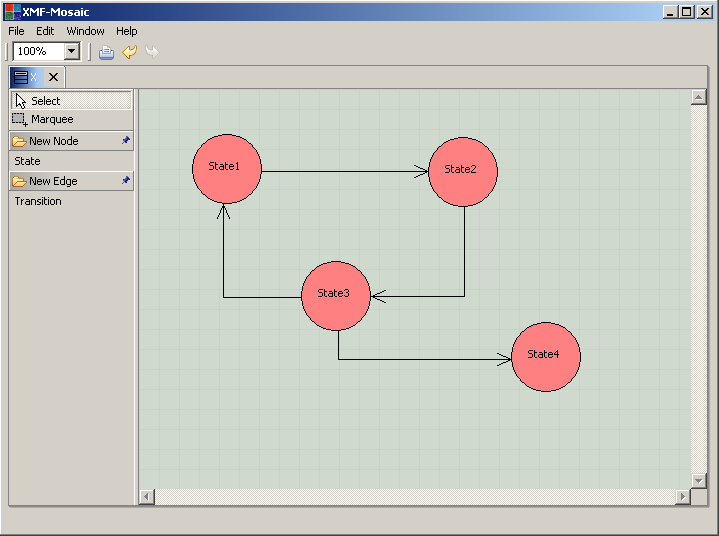
\includegraphics[width=16cm]{ConcreteSyntax/figures/stateMachineTool.png}
\caption{}
\label{stateMachineTool}
\end{center}
\end{figure}

\section{Conclusion}

In order to support the rapid creation of concrete syntaxes for a modelling language, higher level modelling languages are required. This chapter has described XBNF, a language for modelling textual syntaxes. In order to model diagrammatical syntaxes, a framework for modelling common diagrammatic primitives is required, along with a language for describing how the diagrammatic syntax is synchronised with the underlying abstract syntax model of the language.  In chapter \ref{mappingchapter} XSync is introduced which is a declarative language for defining the synchronisation of data and languages.  XSync can be used to succinctly define the types of synchronisations between abstract and concrete syntax discussed in this chapter.
